\section{Diseño y Construcción de la Computadora de Vuelo}

% Acá se da una introducción breve de esta sección, es decir, hay que explicar qué es lo que se va a mencionar acá. Se pone en contexto.

% En esta sección se describe lo que tiene la placa, es decir:
% - Cuáles son las funcionalidades que tiene la placa.
% - Arquitectura general de la placa (algo tipo diagrama en bloques).
% - Criterios tenidos en cuenta para la selección de los componentes (AEC-Q100 y pedidos del laboratorio).
% - Circuitos que implementan cada funcionalidad: selección de componentes, interfaz de comunicación con el micro y circuito diseñado.
% - Circuito completo y PCB <- Acá mencionar el motivo por el que se hizo el PCB de 4 layers y el motivo por el que todos los componentes van de un solo lado.

En esta sección se presentan los criterios tenidos en cuenta para el diseño y la construcción de la computadora de vuelo. Se presentan cuáles son las funcionalidades de la placa y los circuitos que se implementaron para cumplir con estas. Además, se muestra el análisis de la selección de distintos componentes como sensores y circuitos integrados.

%\subsection{Requerimientos y Diseño General}

%\subsubsection{Implementación de Técnicas de Redundancias}

%Uso de un bus de comunicaciones TDMA, utilizado para intercambiar información y realizar algoritmos de votación. Debe poder usarse para implementar una sincronización entre nodos, en caso de que sea necesario.



%Algunos trabajos tienen salidas de control directa sobre los acutadores, la computadora de vuelo debe permitir esto.\\

%La computadora de vuelo requiere interfaces de comunicación con sensores.

%\textbf{{\color{red} COMPLETAR}}

%\subsubsection{Funcionalidades Generales}

%\textbf{{\color{red} COMPLETAR}}

\subsection{Funcionalidades y Diagrama en Bloques}

% Acá lo que hago es mencionar cuáles son las necesidades con las que tengo que cumplir con la placa y después muestro un diagrama en bloques. Todavía no doy ningún circuito, es todo a nivel de sistema.

% Procesa datos de los sensores
% Actúa sobre los motores
% Administra interfaces de comunicación externa (CAN, UART, I2C, SPI, USB, SWD)
% Calcular la ley de control
% Almacenamiento de datos recolectados por la computadora de vuelo, ya sea del vuelo o de la aplicación.
% LEDs indicadores de propósito general.
% Pulsadores para debugging y pruebas de propósito general.

La computadora de vuelo tiene la tarea esencial de adquirir las mediciones de los sensores, procesar dichos datos, y realizar el control de los diversos aspectos del vehículo, fundamentalmente de los motores. Las funcionalidades de la computadora de vuelo son las siguientes:

\begin{enumerate}
    \item Adquirir datos de sensores.
    \item Cálculo de la estimación de la pose y de la ley de control.
    \item Actuación sobre los motores.
    \item \textbf{{\color{red} FALTA ALGUNA FUNCIONALIDAD DE TOLERANCIA A FALLAS}}
    \item Control de LEDs indicadores de propósito general.
    \item Comunicación a través de distintas interfaces, con módulos y sensores externos a la placa.
    \item Loggeo de datos.
\end{enumerate}

\begin{figure}[H]
    \centering
    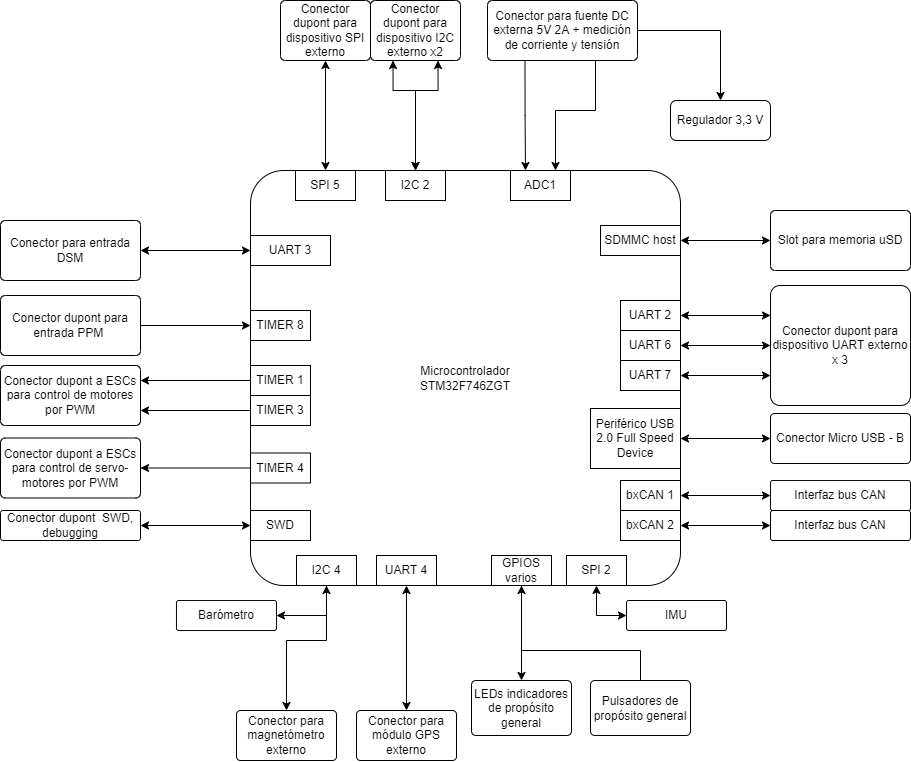
\includegraphics[width=\textwidth]{img/diagrama_en_bloques_computadora_de_vuelo.png}
    \caption{Diagrama en bloques de la computadora de vuelo.}
    \label{fig:diagrama_en_bloques_computadora_de_vuelo}
\end{figure}

\textbf{{\color{red} COMPLETAR}}

\subsection{Criterios Generales Para la Selección de Componentes}

% Acá no se dan justificaciones de algún circuito en particular, sino que se dan justificaciones que aplican a todos los bloques. Por ejemplo, el tema del AEC-Q100 y los pedidos del laboratorio, como los pines dupont, etc.

Para el diseño y la implementación de cada circuito, se tuvieron en cuenta distintas necesidades particulares para cada uno de ellos. A su vez, hay ciertos criterios y que son comunes a todos los circuitos. Estos se mencionan a continuación.

\subsubsection{Uso de Componentes de Grado Automotriz}

Una de las premisas de cualquier trabajo de desarrollo de electrónica, consiste en que este sea de un bajo costo. Gracias al avance de la tecnología, en los últimos años se han ido abaratando los costos de fabricación de chips y componentes electrónicos. Haciendo una búsqueda rápida en sitios web de distintos proveedores de componentes puede encontrarse que existe una gran variedad de estos, como sensores y microcontroladores, a precios razonables.

En el caso particular de sistemas críticos, el aspecto más importante y fundamental es el de la confiabilidad. Generalmente este requerimiento impacta en el costo del desarrollo, ya que la confiabilidad suele traer consigo altos costos de fabricación. Por ejemplo, % AGREGAR EJEMPLOS DE COMPONENTES USADOS EN AVIONES.

% ENTONCES, SE QUIERE HACER ALGO SAFETY-CRITICAL PERO DE BAJO COSTE. ==> MENCIONAR LA OFERTA DE COMPONENTES AUTOMOTRIZ Y HABLAR DE AEC-Q100

\textbf{{\color{red} COMPLETAR}}

\subsubsection{Requerimientos de Conectores}

La computadora de vuelo cuenta con una serie de conectores que permiten el agregado de módulos externos. Algunos de esos conectores fueron seleccionados por una necesidad del LAR, con el objetivo de tener compatibilidad con distintos módulos que son comúnmente utilizados con otras computadoras de vuelo que fueron desarrolladas en el laboratorio. Estos serán mencionados en las secciones correspondientes.

%\subsection{Circuitos Implementados}
\subsection{Microcontrolador}

% Acá sí, va una subsubsection por cada bloque, por ejemplo microcontrolador, IMU, Barómetro, bus CAN, Tarjeta Micro SD, Interfaz USB, etc.

A continuación se describe cada una de las partes del circuito que conforman a la computadora de vuelo. Además de los criterios generales ya mencionados, se mencionan los criterios particulares tenidos en cuenta para cada parte del circuito.

%\subsubsection{Microcontrolador}
\subsubsection{Selección del Componente}

En la versión anterior de la computadora de vuelo, se utilizó un microcontrolador del fabricante ST, en particular el modelo STM32F722. Este cuenta con un procesador ARM Cortex-M7, que puede utilizarse con una frecuencia máxima de 216 MHz. Cuenta con unidad de punto flotante integrada. Además, cuenta con 512 KB de memoria flash y 256 KB de memoria RAM.

A todas las funcionalidades de la computadora de vuelo, en este trabajo se le suman los aspectos relacionados a la tolerancia a fallas. A su vez, se tiene la necesidad de integrar otras funcionalidades que llevan consigo una gran carga computacional. Estas pueden ser propias de la aplicación del vehículo o bien relacionadas a mejorar los algoritmos de navegación y control. Para la versión desarrollada en este trabajo, se buscó actualizar el microcontrolador a uno con mayor rendimiento, sin perder de vista la necesidad de mantener un costo reducido.

Se buscó un microcontrolador del mismo fabricante ST, de manera de tener retrocompatibilidad en el desarrollo del firmware con la versión anterior. De esta forma, muchos de los módulos de firmware que ya se encuentran desarrollados pueden reutilizarse en esta nueva versión. Con estos requerimientos, se analizaron las distintas ofertas del mercado. Además de los aspectos mencionados, se tuvieron en cuenta los periféricos que ofrecía cada modelo, junto con las capacidades de memorias flash y RAM. Se buscó mantener las capacidades de estas memorias en valores similares a las de la versión anterior de la computadora de vuelo.

Como primera opción surgió la posibilidad de seleccionar alguno de los microcontroladores de la serie STM32H7. Estos cuentan con procesdaores ARM Cotex-M7, además de que pueden llegar a velocidades entre 400 MHz y 550 MHz \cite{AN5293} y por ende llegar hasta a duplicar la performance respecto de la versión anterior de la computadora de vuelo. En la tabla \ref{tab:comparacion_MCUs} se muestran distintos modelos que fueron considerados durante la selección del microcontrolador.

\begin{table}[H]
    \centering
    \begin{tabular}{|c||c|c|c|c|c|c|}
        \hline
                        & STM32F722 & STM32H723ZG & STM32H743 & STM32H753 & STM32H735ZG \\
        \hline
        Flash [kB] & 512 & 1024 & \cellcolor{green!25}1024/2048 & \cellcolor{green!25}2048 & 1024\\
        \hline
        SRAM [kB]  & 256 & 564 & \cellcolor{green!25}1024 & \cellcolor{green!25}1024 & 564\\
        \hline
        Freq [MHz] & 216 & \cellcolor{green!25}550 & 480 & 480 & \cellcolor{green!25}550\\
        \hline
        UART & 4 & \cellcolor{green!25}6 & 4 & \cellcolor{green!25}6 & \cellcolor{green!25}6\\
        \hline
        USART & 4 & \cellcolor{green!25}5 & 4 & \cellcolor{green!25}5 & \cellcolor{green!25}5\\
        \hline
        SPI & 5 & \cellcolor{green!25}6 & \cellcolor{green!25}5/6 & \cellcolor{green!25}6 & \cellcolor{green!25}6\\
        \hline
        I2C & 3 & \cellcolor{green!25}5 & 4 & 4 & \cellcolor{green!25}5\\
        \hline
        CAN & 1 & \cellcolor{green!25}3 & 2 & \cellcolor{green!25}3 & \cellcolor{green!25}3\\
        \hline
        ADC & 3x12b, 24ch & \makecell{2x16b, 22 ch; \\ 1x12b, 12 ch} & \cellcolor{green!25}\makecell{3x16b, \\ 16/28/32ch} & \makecell{1x12b, 12ch \\ 2x16b, 18ch} & \makecell{1x12b, 12ch \\ 2x16b, 16ch}\\
        \hline
        Timers & \makecell{18: 16b x 16, \\ 32b x 2} & \cellcolor{green!25}\makecell{21: 16b x 17, \\ 32b x 4} & \makecell{14: 16b x 12, \\ 32b x 2} & \cellcolor{green!25}\makecell{21: 16b x 17, \\ 32b x 4} &\cellcolor{green!25} \makecell{21: 16b x 17, \\ 32b x 4}\\
        \hline
        SDMMC & \cellcolor{green!25}2 & \cellcolor{green!25}2 & \cellcolor{green!25}2 & \cellcolor{green!25}2 & \cellcolor{green!25}2\\
        \hline
        longevidad & \cellcolor{green!25}01/2033 & \cellcolor{green!25}01/2033 & \cellcolor{green!25}01/2033 & \cellcolor{green!25}01/2033 & \cellcolor{green!25}01/2033\\
        \hline
        AEC-Q100 & No & No & No & No & No\\
        \hline       
    \end{tabular}
    \caption{Se muestra la comparación de las distintas alternativas que fueron tenidas en cuenta para la selección del mircocontrolador. En verde se destaca el componente que tiene las mejores características para cada fila. El modelo STM32F722 corresponde al modelo utilizado en la versión 3 de la computadora de vuelo.}
    \label{tab:comparacion_MCUs}
\end{table}

Todos los microcontroladores de la serie STM32H7 presentan mejoras en cuanto a frecuencia de operación, memoria flash y RAM. Sumado a esto, la gran mayoría de estos microcontroladores se encuentran dentro del programa \textit{Longevity Commitment} \cite{longevity_ST}. El fabricante ST se compromete a mantener la producción de los componentes que se encuentren dentro de este programa durante un período determinado. Todos los microcontroladores de la tabla \ref{tab:comparacion_MCUs} tienen un periódo de fabricación de 10 años asegurado por ST, finalizando en 01/2033. Este aspecto es de especial interés teniendo en cuenta la posible necesidad futura de fabricar nuevas placas de la computadora de vuelo.\\

\textbf{{\color{red} COMPLETAR POR QUÉ NO SE ELEIGIÓ UNO AEC-Q100, QUE ES PORQUE NO HABÍA CORTEX M7 DE ST QUE SEA AEC-Q100}}

\textbf{{\color{red} COMPLETAR LA JUSTIFICACIÓN DE QUE SE ELIGIÓ UN MICROCONTROLADOR DIFERENTE DEBIDO A LA CRISIS Y FALTANTE DE CHIPS}}

% Acá lo importante es decir que se quería elegir un controlador más potente que la choriboard III, algún STM32H7. Mencionar por qué STM32, que es porque ellos vienen trabajando con esos microcontroladores. Luego explicar que debido al faltante y la crisis, se tuvo que elegir otro controlador. También, mencionar que el que se eligió tiene 10 años de garantía de fabricación, lo que favorece la longevidad.

La selección del microcontrolador utilizado se vio limitada por la disponibilidad de componentes encontrada durante el período de desarrollo del circuito. El microcontrolador seleccionado fue el STM32F746ZG. Este cuenta con un procesador ARM-Cortex M7, 1024 kB de memoria flash y 320 kB de memoria SRAM. Un aspecto relevante de este microcontrolador es que cuenta con 2 interfaces CAN. El bus CAN se utilizará para establecer las comunicaciones relevantes a los algoritmos de tolerancia a fallas. La posibilidad de contar con 2 interfaces CAN trae consigo el hecho de que el bus no sea un punto singular de falla.

% Mencionar cómo se asignaron los distintos timers para su uso en la aplicación.


% Mencionar cómo se asignaron las interrupciones externas de gpios.

% Acá también hay que mencioanr todos los cálculos y justificaciones para la selección del cristal, tanto de 12 MHz como el de 32 kHz. Poner todo lo que tengo, esta sección tiene muchísimo para mostrar.

\textbf{{\color{red} COMPLETAR}}

%\subsection{Otros Circuitos Implementados}

%\subsubsection{Sensor IMU}

\subsubsection{Requerimientos del Componente}

\textbf{{\color{red} COMPLETAR}}

% acá van todos los capacitores de desacople, etc

\subsubsection{Cristal Externo}

\textbf{{\color{red} COMPLETAR}}

\subsubsection{Cristal para RTC}

\textbf{{\color{red} COMPLETAR}}

\subsection{Sensor IMU}

La unidad de medición inercial, IMU por sus siglas en inglés, es el sensor principal utilizado por la computadora de vuelo. Este consiste en un circuito integrado que contiene una serie de sensores inerciales, en particular acelerómetros y giróscopos. Los acelerómetros se utilizan para realizar mediciones de aceleración lineal y los giróscopos para medir velocidad angular. A partir de estas mediciones, se pueden aplicar distintos algoritmos de procesamiento para obtener una estimación de la posición y orientación del vehículo. Las mediciones de aceleración lineal y de velocidad angular que entrega la IMU son referidas a una terna solidaria al componente, como se muestra en la figura \ref{fig:IMU_ejes}.

\begin{figure}[H]
    \centering
    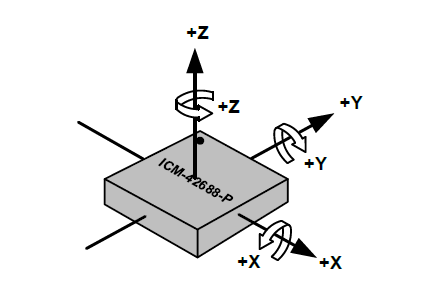
\includegraphics[width=0.4\textwidth]{img/IMU_ejes.png}
    \caption{Todas las mediciones que entrega el sensor son realtivas a una terna solidaria a este. La imagen se extrajo de \cite{ICM42688pDatasheet}.}
    \label{fig:IMU_ejes}
\end{figure}

Los acelerómetros y giróscopos de la IMU utilizada en este trabajo, se construyen utilizando la tecnología MEMS: \textit{Microelectromechanical Systems}. Utilizando técnicas de fabricación de circuitos integrados, se construyen los acelerómetros y giróscopos, integrando en el silicio partes que son móviles. En la figura \ref{fig:MEMS_acelerometro}, se muestra una imagen tomada con un microscopio electrónico de un acelerómetro MEMS. Lo que se observa en este caso, es que en el mismo silicio se integra una masa llamada \textit{proof-mass}, la cual se encuentra sujeta al sustrato a través de dos resortes.

\begin{figure}[H]
    \centering
    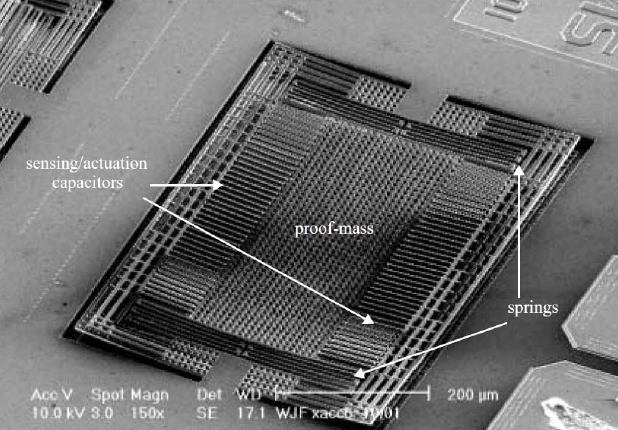
\includegraphics[width=0.6\textwidth]{img/MEMS_acelerometro.png}
    \caption{Fotografía tomada de un acelerómetro construido con tecnología MEMS. La imagen se extrajo de \cite{zhang2010sensing}. }
    \label{fig:MEMS_acelerometro}    
\end{figure}

Una aceleración sobre el componente genera que la masa del acelerómetro se mueva. Estos desplazamientos producen una variación en la capacidad existente entre el sustrato y la masa, lo que lleva a una variación de la tensión entre ambos. Esta diferencia de potencial variable es medida por un circuito dentro del chip, y que luego se utiliza para generar las mediciones de aceleración.\\

El acelerómetro puede modelarse de manera simple, como un sistema mecánico con una masa, un resorte y un amortiguador \cite{zhang2010sensing}, como se muestra en la figura \ref{fig:acelerometro_modelo}.

\begin{figure}[H]
    \centering
    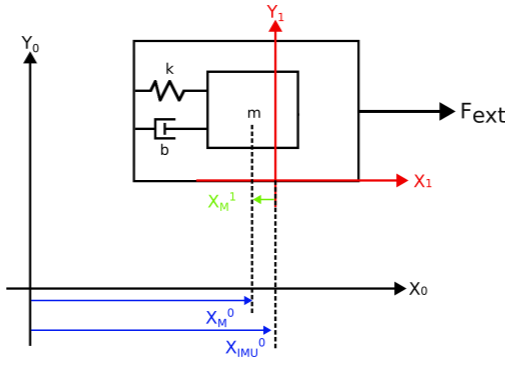
\includegraphics[width=0.5\textwidth]{img/acelerometro_modelo.png}
    \caption{Sistema mecánico simplificado del acelerómetro.}
    \label{fig:acelerometro_modelo}    
\end{figure}

La terna 0 corresponde a una terna inercial, mientras que la terna 1 es no inercial, solidaria al movimiento del acelerómetro. Cabe aclarar que tal como se mencionó, la masa se encuentra sujeta al sustrato solamente a través del resorte. El elemento amortiguador representa pérdidas de energía, causadas por rozamiento con el aire o de la propia estructura electromecánica. Se puede resolver el sistema mecánico, tomando como coordenadas generalizadas $q_1 = X_{IMU}^0$ y $q_2 = X_M^1$. Sin considerar efectos de la gravedad, se llega a la ecuación \eqref{eq:acelerometro_segundo_orden}. Este es un sistema de segundo orden, donde la entrada es la aceleración del acelerómetro y la salida es el desplazamiento de la masa respecto de la terna solidaria al acelerómetro. 

\begin{equation}
    \ddot{X_M^1} + \frac{b}{m} \dot{X_M^1} + \frac{k}{m} X_M^1 = -\ddot{X_{IMU}^0}
    \label{eq:acelerometro_segundo_orden}
\end{equation}

Como resultado interesante, se observa que el sistema es de segundo orden, típicamente con respuesta sub-amortiguada. Algunos fabricantes de estos sensores indican en sus hojas de datos, un valor de frecuencia de resonancia. Este valor resulta de interés ya que si se excita al sensor con frecuencias cercanas a la resonancia, dejará de funcionar como dispositivo para medir la aceleración lineal. Por otro lado, a muy bajas frecuencias se puede despreciar la velocidad de la masa y luego se obtiene una relación directa entre la aceleración del acelerómetro y el desplazamiento de la masa, ecuación \eqref{eq:relacion_aceleracion_despalzamiento}.

\begin{subequations}
	\begin{align}
        \ddot{X_M^1} &\approx 0\\
        \dot{X_M^1} &\approx 0\\
        \frac{k}{m} X_M^1 &\approx -\ddot{X_{IMU}^0}
	\end{align}
    \label{eq:relacion_aceleracion_despalzamiento}
\end{subequations}

El desplazamiento de la masa produce una variación de la capacidad entre esta y el sustrato. Esta capacidad es utilizada para medir una varaición de tensión \cite{zhang2010sensing}. El circuito medido puede modelarse como en la figura \ref{fig:acelerometro_sensado_capacitivo}.

\begin{figure}[H]
    \centering
    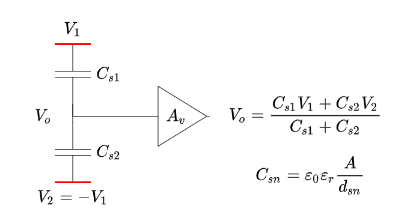
\includegraphics[width=0.5\textwidth]{img/acelerometro_sensado_capacitivo.png}
    \caption{Circuito equivalente que mide el desplazamiento de la masa. Las tensiones $V1$ y $V2$ representan señales de tensión aplicadas por un circuito externo. El movimiento de la masa modifica la capcidad y por ende la tensión medida.}
    \label{fig:acelerometro_sensado_capacitivo}    
\end{figure}

Se puede resolver este circuito y llegar a que existe una relación lineal entre la tensión $Vo$ y el desplazamiento de la masa $\Delta d$, ecuación \eqref{eq:tension_salida_acelerometro}. En \cite{zhang2010sensing} puede encontrarse la demostración completa. En la ecuación, $d_0$ representa la separación de reposo entre el sensor y el sustrato y $\Delta d$ la variación de la separación.

\begin{equation}
    V_{o} = \frac{\Delta d}{d_0} V_1
    \label{eq:tension_salida_acelerometro}
\end{equation}

\textbf{{\color{red} COMPLETAR UN ANÁLISIS SIMILAR PARA EL GIRÓSCOPO}}

Se hizo una búsqueda de las distintas alternativas existentes para este tipo de sensores. A partir de leer las hojas de datos de distintos fabricantes, se encontró que los parámetros típicamente especificados, tanto para los acelerómetros como para los giróscopos, son los siguientes:

\begin{itemize}
    \item \textit{Full-scale range}
    \item \textit{Sensitivity}
    \item \textit{Scale factor error}
    \item \textit{Scale factor error vs temp}
    \item \textit{Offset}
    \item \textit{Offset vs temp}
    \item \textit{Offset vs time}
    \item \textit{Noise}
\end{itemize}

El primero de ellos, el \textit{Full-scale range} es el rango de medición del sensor. Para los acelerómetros se suele especificar en un rango de $\pm n \times g$, donde $n$ es algún entero y $g$ representa la aceleración de la gravedad. Para los giróscopos, se especifica como $\pm n \times dps$, donde $dps$ significa \textit{degrees-per-second}.\\

El parámetro \textit{Sensitivity} hace referencia a la resolución. En algunas hojas de datos este parámetro puede encontrarse con unidades de $LSB/g$ para los acelerómetros y en $LSB/dps$ para los giróscopos. Este valor puede resultar confuso de entender, ya que lo que informa es la cantidad de bits por $g$ o la cantidad de bits por $dps$. En la figura \ref{fig:ICM_42688_datasheet} se muestra una captura de la hoja de datos del sensor seleccionado, el ICM42688p. 

\begin{figure}[H]
    \centering
    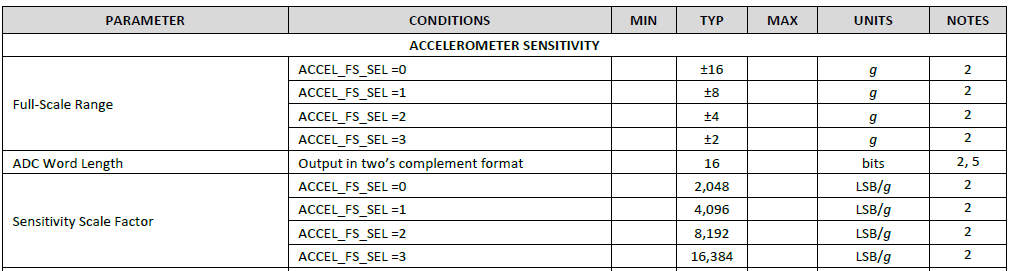
\includegraphics[width=\textwidth]{img/ICM_42688_datasheet.png}
    \caption{Extracto de la hoja de datos del sensor ICM42688p. Se muestra parte de las especificaciones para los acelerómetros.}
    \label{fig:ICM_42688_datasheet}    
\end{figure}

La imagen muestra que el sensor permite seleccionar distintos rangos de escala para las mediciones del acelerómetro. Por ejemplo, si se selecciona el rango $\pm 2g$, la hoja de datos especifica una resolución de $16384 \ LSB/g$. Una mejor forma de entender este parámetro sería si se considera la inversa, es decir, la resolución del ADC. En este caso sería de $61.04 \ 10^{-6} \ g$. Luego para un rango de $\pm 4g$ la resolución es de $8192 \ LSB/g$, es decir, $122.07 \ 10^{-6} \ g$. Este valor es el doble del anterior y tiene sentido dado que se está midiendo un rango mayor de aceleraciones utilizando la misma cantidad de bits, en este caso 16 según lo especificado en la hoja de datos.\\

Para entender los parámetros, \textit{scale factor error}, \textit{offset} y \textit{noise} se plantea un modelo sencillo de medición, tanto para acelerómetros como para giróscopos \cite{borodacz2022review}. Este se presenta en la ecuación \eqref{eq:medicion_vs_real}, donde $S$ es el \textit{scale factor error}, $\omega_b(t)$ es el \textit{offset} el cual es variable con el tiempo, $\eta \sim \mathcal{N}(0,\sigma^2)$, $\omega_m$ es el valor medido y $\omega$ sería la velocidad angular verdadera para el giróscopo.

\begin{equation}
    \omega_m = (1+S)\omega + \omega_b (t) + \eta
    \label{eq:medicion_vs_real}
\end{equation}

A su vez, en las hojas de datos se especifica la dependencia de estos parámetros con el tiempo y con la temperatura, como es el caso del \textit{scale factor error}.\\

Para tener un criterio de selección del sensor IMU, se siguió el análisis planteado en \cite{borodacz2022review}. Este paper presenta un análisis de los parámetros de los acelerómetros y grióscopos y su impacto en las estimaciones de posición en sistemas de navegación inercial (INS). En este se concluye que los parámetros más importantes para la selección del sensor son:

\begin{itemize}
    \item Estabilidad del offset de los acelerómetros (Offset vs time).
    \item Estabilidad del offset de los giróscopos (Offset vs time).
    \item Ruido de los giróscopos (Noise).
    \item Error de escala del giróscopo (Scale factor error).
\end{itemize}

Se buscaron modelos de IMUs de distintos fabricantes, para comparar características. Existe una gran cantidad de fabricantes y de componentes para seleccionar. Se buscaron componentes que sean accesibles y que no tengan un costo muy elevado. Existen IMUs de una excelente calidad, pero que tienen precios que no están al alcance (cientos o miles de dólares). Con este criterio, se realizó una comparación entre distintos modelos de sensores. En la tabla \ref{tab:comparacion_IMUs} se muestra una comparación de los distintos sensores considerados. Sumado a esto, se tuvo en consideración otro aspecto que fue mencionado anteriormente, la longevidad del componente.

\begin{table}[H]
    \centering
    \begin{tabular}{|c||c|c|c|c|c|}
        \hline
                        & ICM42688 & LSM6DSR & IIM-42652 & BMI088 & ASM330LHHX\\
        \hline
        $b_{accel}a(t)$ & N/A      & N/A     & N/A       & N/A    & \cellcolor{green!25}40 $\mu$ g\\
        $b_{gyro}(t)$   & N/A      & N/A     & N/A       & \cellcolor{green!25}2°/h    & 3°/h\\
        $\eta_{gyro}$   & \cellcolor{green!25}$2.8 mdps/\sqrt{Hz}$ & $5 mdps/\sqrt{Hz}$ & $3.8 mdps/\sqrt{Hz}$ & $14 mdps/\sqrt{Hz}$ & $5 - 12 mdps/\sqrt{Hz}$\\
        $S_{gyro}$ & \cellcolor{green!25}$0.5 \%$ & $1 \%$ & \cellcolor{green!25}$0.5 \%$ & $1 \%$ & $2 \%$\\
        \hline
        longevidad & N/A & N/A & 10 años, dic. 2020 & N/A & \cellcolor{green!25}15 años, mayo 2022\\
        AEC-Q100 & No & No & No & No & \cellcolor{green!25}Sí\\
        \hline       
    \end{tabular}
    \caption{Se muestra la comparación de las distintas alternativas que fueron tenidas en cuenta para la selección del sensor. En verde se destaca el componente que tiene las mejores características para cada parámetro.}
    \label{tab:comparacion_IMUs}
\end{table}

Lo primero que llama la atención es el hecho de que muchos de los sensores no especifican estos parámetros. Solamente una de las alternativas consideradas tiene disponible toda la información en su hoja de datos. Esto dificulta mucho la selección de un componente. A priori, se selecciona el sensor ASM330LHHX por el hecho de ser el único que ofrece toda la información en su hoja de datos, además de ser de grado automotriz y tener una longevidad garantizada de 15 años. Teniendo en cuenta aspectos de confiabilidad, resulta esencial el hecho de conocer los parámetros del sensor.\\

Durante la selección del sensor hubo otro aspecto importante que se tuvo en cuenta y es el hecho de la compatibilidad con el software desarrollado por el laboratorio, para computadoras de vuelo anteriores a la de este trabajo. La versión anterior contaba con un sensor IMU ICM20602, del fabricante TDK. El laboratorio cuenta con bibliotecas de código ya desarrolladas para este sensor. Este presentó excelentes resultados, lo que sienta un antecedente importante en la selección de componentes del mismo fabricante. En la tabla \ref{tab:comparacion_IMUs_TDK} se muestra una comparación entre el sensor anterior ICM20602 y el sensor seleccionado ICM42688.

\begin{table}[H]
    \centering
    \begin{tabular}{|r||c|c|}
        \hline
         & ICM20602 & ICM42688 \\
        \hline
        Año & 2016 & 2021\\
        \hline
        \multicolumn{3}{|c|}{Giróscopos}\\
        \hline
        Full Scale Range[dps] & $\pm 250/500/1000/2000$ & $\pm 15/31/62/125/250/500/1000/2000$\\
        Scale Factor Error[\%] & $1.0$ @ 25°C & $0.5$ @ 25°C\\
        Scale factor error vs temp[\%/°C] & $0.016$ @ -40°C - 85 °C & $0.005$ @ 0°C - 70 °C\\
        Offset[dps] & $\pm 1$ & $\pm 0.5$\\
        Offset vs temp[dps/°C] & $0.01$ & $0.005$\\
        Offset vs time[°/h] & N/A & N/A\\
        Noise[$mdps/\sqrt{Hz}$] & $4$ & $2.8$\\
        \hline
        \multicolumn{3}{|c|}{Acelerómetros}\\
        \hline
        Full Scale Range[g] & $\pm 2/4/8/16$ & $\pm 2/4/8/16 $\\
        Scale Factor Error[\%] & $1.0$ @ 25°C & $0.5$ @ 25°C\\
        Scale factor error vs temp[\%/°C] & $0.012$ @ -40°C - 85 °C & $0.005$\\
        Offset[mg] & $\pm 25$ & $\pm 20$\\
        Offset vs temp[mg/°C] & X,Y: $\pm 0.5$, Z: $\pm 1$ & $\pm 0.15$\\
        Offset vs time[$\mu$g/h] & N/A & N/A\\
        Noise[$\mu g/\sqrt{Hz}$] & $100$ & X,Y: $65$, Z: $70$\\        
        \hline       
    \end{tabular}
    \caption{Se muestra la comparación del sensor ICM20602 y el sensor seleccionado ICM42688.}
    \label{tab:comparacion_IMUs_TDK}
\end{table}

Para el diseño del circuito se siguieron las recomendaciones en la hoja de datos del componente. Este sugiere incluir una serie de capacitores de desacople en los terminales de alimentación del componente. Se elige utilizar una comunicación SPI en modo esclavo, donde el maestro es el microcontrolador. La interfaz SPI permite obtener velocidades de transferencia más altas que utilizando otras interfaces como I2C. El circuito completo puede encontrarse en el \nameref{appendix:circuito_esquematico}.\\

Dado que el sensor IMU es un esclavo en la comunicación SPI, este solo puede comunicarse con el microcontrolador, el maestro, cuando este último le solicite la información. La IMU genera lecturas de sus aceleróemtros y giróscopos de manera periódica. De manera de que la IMU pueda informar al microcontrolador el momento en el que generó una nueva lectura, el sensor dispone de una salida digital que puede conectarse a una entrada digital del microcontroldor. De esta forma, cuando el microcontrolador detecta un cambio de nivel en esa entrada digital, procede a pedirle el dato generado a través de la comunicación SPI. En la figura \ref{fig:IMU_SPI} se muestra un esquema de la conexión entre el controlador y el sensor IMU.

\begin{figure}[H]
    \centering
    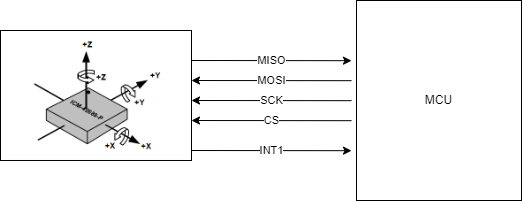
\includegraphics[width=0.8\textwidth]{img/IMU_SPI.png}
    \caption{Líneas de comunicación entre la IMU y el microcontrolador.}
    \label{fig:IMU_SPI}    
\end{figure}

%\subsubsection{Barómetro}
\subsection{Barómetro}

Al igual que la IMU, el barómetro que se utiliza corresponde a un sistema MEMS. Este sensor se utiliza para estimar la altura del vehículo respecto del suelo, a partir de mediciones de presión. En particular, los barómetros MEMS cuentan con un sistema capaz de medir la presión absoluta, es decir respecto al 0 de presión. Estos cuentan con una cavidad integrada dentro del chip que se encuentra (idealmente) a presión 0. A través de un proceso llamado \textit{anodic bonding} \cite{baro_1}\cite{baro_2} se construye esta cavidad dentro del chip, la cual se encuentra sellada a una presión muy baja, en comparación con las presiones que se esperan medir utilizando el componente. Para medir la presión, se coloca una membrana sobre la cavidad. En la figura \ref{fig:MEMS_barometro} se puede apreciar el efecto de la presión externa sobre la membrana, la presión atmosférica. Sobre las zonas de color violeta, se colocan resistores de efecto piezoresistivo. En consecuencia, la deformación de la membrana genera tensión sobre estos, modificando su resistencia.

\begin{figure}[H]
    \centering
    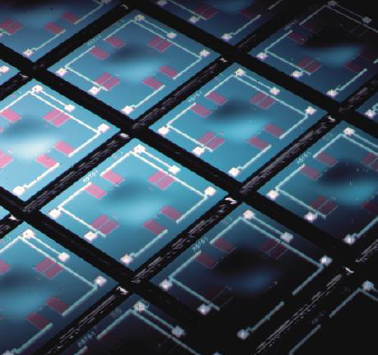
\includegraphics[width=0.4\textwidth]{img/MEMS_barometro.png}
    \caption{Sensores de presión sobre una oblea de silicio \cite{baro_1}.}
    \label{fig:MEMS_barometro}
\end{figure}

Los resistores se conectan en configuración puente de Wheatstone, de manera tal de que la presión comprime a dos de los resistores y estira a los otros dos \cite{baro_3}. En \eqref{eq:barometro_wheatstone} se despeja la relación entre la variación de tensión y la variación de la resistencia. Como se observa, la realación es proporcional.

\begin{figure}[H]
    \centering
    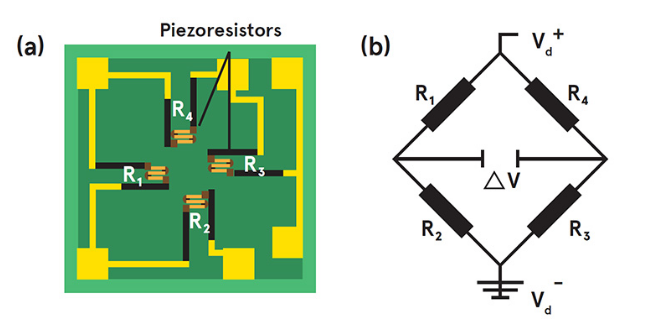
\includegraphics[width=0.7\textwidth]{img/barometro_wheatstone.png}
    \caption{Puente de Wheatstone conformado por los resistores del sensor de presión. La imagen se extrajo de \cite{baro_3}.}
    \label{fig:barometro_wheatstone}
\end{figure}

\begin{subequations}
    \begin{align}
        \Delta V &= (V_d^+ - V_d^-) \left[ \frac{R_2}{R_2 + R_1} - \frac{R_3}{R_3 + R_4} \right]\\
        R_1 &= R_3 = R - \Delta R\\
        R_2 &= R_4 = R + \Delta R\\
        \Delta V &= (V_d^+ - V_d^-) \frac{\Delta R}{R}
    \end{align}
    \label{eq:barometro_wheatstone}
\end{subequations}

En la aplicación del vehículo aéreo, el barómetro se utiliza con el fin de medir la altura del vehículo, respecto de una altura inicial. La forma de medir la altitud a través de la presión es utilizando la ecuación de los gases nobles para el aire \cite{cavcar2000international}. En las ecuaciones \eqref{eq:gases_nobles} se obtiene una expresión para la presión, en función de la densidad del aire, la constantes de los gases y la masa molar del aire.

\begin{subequations}
    \begin{align}
        P V &= n R T\\
        n &= \frac{m}{M}\\
        P V &= \frac{m}{M} R T\\
        P &= \frac{m}{V} \frac{R T}{M}\\
        P &= \rho \frac{R T}{M} \label{eq:presion_gas_nobles}
    \end{align}
    \label{eq:gases_nobles}
\end{subequations}

Luego, utilizando la condición hidrostática, la presión es la ejercida por la columna de aire \cite{cavcar2000international}. En la condición hidrostática de la ecuación \ref{eq:condicion_hidrostatica} se puede despejar la densidad del aire y reemplazarla en \eqref{eq:presion_gas_nobles}. Finalmente, se obtiene la ecuación diferencial de \eqref{eq:presion_diferencial}.

\begin{equation}
    dp = -\rho g dh
    \label{eq:condicion_hidrostatica}
\end{equation}

\begin{equation}
    \frac{dP}{P} = - \frac{g M}{R T} dh
    \label{eq:presion_diferencial}
\end{equation}

Esta ecuación puede integrarse a ambos lados para hallar la relación entre la presión y la altura. Todos los términos de la ecuación \eqref{eq:presion_diferencial} son constantes, a excepción de la temperatura. Según el modelo \textit{International Standard Atmosphere} (ISA), se modela la relación entre la temperatura y la altitud, según la ecuación \eqref{eq:ISA_temperatura}. Esta relación es válida solamente hasta la estratósfera.

\begin{subequations}
    \begin{align}
        T(h) &= T_0 + L \ h\\
        T(h) &= 288.15 K - h \ 6.5 \ 10^{-3} m/K
    \end{align}
    \label{eq:ISA_temperatura}
\end{subequations}

Finalmente, se obtiene una expresión de la presión en función de la altura, ecuación \eqref{eq:ISA_presion}. 

\begin{subequations}
    \begin{align}
        P(h) &= P_0 \left[ 1 + \frac{L h}{T_0} \right]^{-\frac{M g}{R L}}\\
        P(h) &= 1013.25 \ hPa \left[ 1 - 0.0065 \frac{h}{288.15 K} \right]^{5.2561}
    \end{align}
    \label{eq:ISA_presion}
\end{subequations}

Se puede obtener un modelo más simplificado si se asume una temperatura constante, independiente de la altitud. Se reemplaza en \eqref{eq:presion_diferencial} y resolviendo la ecuación diferencial se obtiene la ecuación \eqref{eq:presion_temp_constante}.

\begin{subequations}
    \begin{align}
        P(h) &= P_0 \ e^{-\frac{g M h}{R T}}\\
        P(h) &= 1013.25 \ hPa \ e^{-\frac{h}{8840.2 m} }
    \end{align}
    \label{eq:presion_temp_constante}
\end{subequations}

Al igual que con el sensor IMU, se hizo una búsqueda de las distintas alternativas. Los parámetros típicamente especificados son los siguientes:

\begin{itemize}
    \item \textit{Full-scale range}
    \item \textit{Absolute Accuracy}
    \item \textit{Relative Accuracy}
    \item \textit{Solder Drift}
    \item \textit{Offset vs temp}
    \item \textit{Offset vs time}
    \item \textit{Noise}
\end{itemize}

Como se puede ver, estos son similares a los de la IMU. Las diferencias se encuentran en los parámetros \textit{Absolute Accuracy}, \textit{Relative Accuracy} y \textit{Solder Drift}.\\

Se puede plantear un mismo modelo de medición según la ecuación \ref{eq:medicion_vs_real} pero para la presión.

\begin{equation}
    P_m = (1+S)P + P_b(t) + \eta
    \label{eq:medicion_presion}
\end{equation}

En el caso de la IMU, el parámetro \textit{scale factor error} se refiere al término $S$ y el \textit{offset} al término $P_b$. En el caso del barómetro, estos valores se encuentran especificados de otra manera. Si se quiere medir una presión $P$, el error de medición será $\Delta P = S \ P + P_b(t) + \eta$. El término $S \ P + P_b(t)$ corresponde al parámetro \textit{absolute accuracy} \cite{baro_4}. Este error es introducido debido a que la cavidad dentro del sensor no se encuentra a presión 0 perfecta, sino que a un pequeño valor \cite{baro_1}. Por otro lado, el término $S \ P$ se lo denomina \textit{relative accuracy}. Este hace referencia a mediciones diferenciales de presión. Algunos barómetros MEMS traen consigo una funcionalidad para realizar una compensación de offset. Esto dejaría como parámetro de interés para mediciones de presión a la \textit{relative accuracy}, la cual hace referencia al error introducido para mediciones de variaciones de presión.\\

El parámetro \textit{solder drfit} se refiere al offset que se introduce por el propio proceso de soldadura \cite{baro_4}. Este offset también puede ser compensado a través de la calibración del barómetro.\\

Se buscaron modelos de barómetros de distintos fabricantes, para comparar características, teniendo en cuenta la accesibilidad y el bajo costo. En la tabla \ref{tab:comparacion_baros} se muestra una comparación de los distintos barómetros considerados. Sumado a esto, se tuvo en consideración otro aspecto que fue mencionado anteriormente, la longevidad del componente.

\begin{table}[H]
    \centering
    \begin{tabular}{|c||c|c|c|c|c|c|}
        \hline
          & BMP390 & BMP581 & ICP-20100 & LPS22HH & ILPS22QSTR & DPS368\\
        \hline
        Full scale range [hPa] & 300 - 1250 & 300 - 1250 & 260 - 1260 & 260 - 1260 & 260 - 1260 ; 260 - 4060 & 300 - 1200\\ 
        absolute acc [hPa] & $\pm 0.5$ & $\pm 0.3$ & $\pm 0.2$ & $\pm 0.5$ & $\pm 0.5$ & $\pm 1$\\
        realtive acc [hPa] & $\pm 0.03$ & $\pm 0.06$ & $\pm 0.01$ & $\pm 0.025$ & $\pm 0.015$ & $\pm 0.06$\\
        \hline
        longevidad & N/A & N/A & N/A & N/A & 10 años, enero 2023 & N/A \\
        AEC-Q100 & No & No & No & No & No & No\\
        \hline       
    \end{tabular}
    \caption{Se muestra la comparación de las distintas alternativas que fueron tenidas en cuenta para la selección del sensor.}
    \label{tab:comparacion_baros}
\end{table}

Las dos alternativas que se evaluaron son los sensores ICP-20100 y el ILPS22QSTR. El primero de ellos presenta las \textit{absolute accuracy} y \textit{relative accuracy} más bajas de entre todas las opciones evaluadas. El sensor ILPS22QSTR presenta características similares y además tiene la particularidad de que el fabricante garantiza su fabricación por 10 años, hasta enero de 2033 \cite{baro_5}. Finalmente el sensor seleccionado fue este último.\\

En cuanto al circuito, en este caso también se tomó como guía el circuito de la hoja de datos del componente. La interfaz de comunicación seleccionada es I2C. Se prefiere utilizar I2C en lugar de SPI ya que puede aprovecharse el uso del mismo bus al que se conecta el barómetro, para conectar otros sensores y dispositivos. De esta manera, se ahorra la cantidad de pistas y conexiones en el diseño del PCB. Si bien I2C es más lento que SPI, las mediciones del barómetro no son tan críticas como las de la IMU. Este sensor, a diferencia de a IMU, no cuenta con una línea de interrupción, por lo que los datos deben obtenerse por \textit{polling} de forma peródica. El circuito completo puede encontrarse en el \nameref{appendix:circuito_esquematico}.

%\subsubsection{Magnetómetro}
\subsection{Magnetómetro}

\textbf{{\color{red} COMPLETAR}}

\subsubsection{Interfaz de Comunicación CAN}
\subsection{Interfaz de Comunicación CAN}

% Como fue mencionado, la computadora de vuelo cuenta con la capacidad de conexión a un bus CAN. La especificación original del protocolo \cite{specification1991bosch} incluye dentro de sus definiciones, la capa física. Cada nodo de un bus CAN se conecta a este a través de 2 cables, los cuales llevan la señal diferencial. Esto se muestra en la figura \ref{fig:conxeion_al_bus_CAN}. Todo el bus CAN se compone de 2 cables que llevan los mensajes a todos los nodos de la red. Esto es así debido a que el bus CAN originalmente fue diseñado para utilizarse en automóviles y reemplazar la enorme cantidad de conexiones entre módulos. El hecho de que se trate de una señal diferencial hace que la comunicación sea robusta, reduciendo las emisiones electromagnéticas generadas por este. A su vez, es común que el bus sea cableado como un par trenzado, lo que atenúa señales de modo común, producto de cualquier acoplamiento. 

% \begin{figure}[H]
%     \centering
%     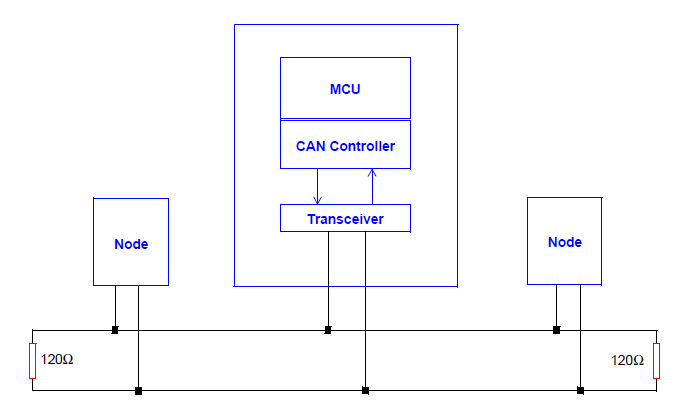
\includegraphics[width=0.5\textwidth]{img/conxeion_al_bus_CAN.png}
%     \caption{La conexión de un nodo al bus es a través de 2 cables que llevan dos señales, CAN-H y CAN-L. La imagen se extrajo de \cite{AN228}.}
%     \label{fig:conxeion_al_bus_CAN}    
% \end{figure}

% Existen muchas versiones del protocolo CAN, en este trabajo se utiliza la versión CAN High Speed. Esta define una velocidad máxima de transferencia de 1 Mbps, para un bus de hasta 40 m de longitud y 30 nodos conectados al mismo bus. Se recomienda que la conexión entre cada nodo y el bus no sea de más de 30 cm. El hecho de poder tener hasta 30 nodos expande las posibilidades de uso del bus, más allá de ser el medio principal de comunicación utilizado para el sistema redundante. Por ejemplo, distintos sensores o incluso actuadores como los motores del vehículo podrían conectarse al bus. {\color{red} Acá tendría que agregar alguna referencia a este uso del bus CAN}.\\

% La impedancia característica del bus debe ser de $120 \ \Omega$. Es común agregar resistores de terminación en ambos extremos, para evitar reflexiones. En algunos casos pueden llegar a encontrarse aplicaciones donde los resistores de terminación se incluyen dentro de alguno de los nodos del bus. Esto no es recomendable, ya que si este se desconecta de forma accidental del bus, todas las comunicaciones entre los demás nodos se verán perjudicadas. Este es el motivo por el cual la computadora de vuelo no incluye este resistor en el circuito.\\

% En la figura \ref{fig:conxeion_al_bus_CAN} se muestran 2 elementos que forman parte del nodo, el \textit{trasnciever} y el \textit{controller}. El primero de ellos forma parte de la capa física y es un circuito que convierte las señales diferenciales del bus en señales de modo común, que luego son transferidas al elemento \textit{controller}. Este componente sirve como interfaz física con el bus.\\

El micronotrolador seleccionado para la computadora de vuelo, cuenta con un \textit{controller} embebido, el periférico bxCAN \cite{STM32F746ZG}. Este cuenta con dos líneas de comunicación con el transciever, CAN TX y CAN RX. En la figura \ref{fig:microcontrolador_transciever} se muestra la comunicación entre transciever, controller y el bus. Cuando se quiere transferir un mensaje a través del bus CAN, el periférico envía un mensaje a través del terminal CAN TX. El transciever lo recibe y lo convierte en una señal diferencial para inyectarlo en el bus. Cuando el nodo recibe un mensaje del bus CAN, el transciever es el que interactúa con el bus y genera una señal de modo común, la cual es enviada a través del terminal CAN RX al microcontrolador.

\begin{figure}[H]
    \centering
    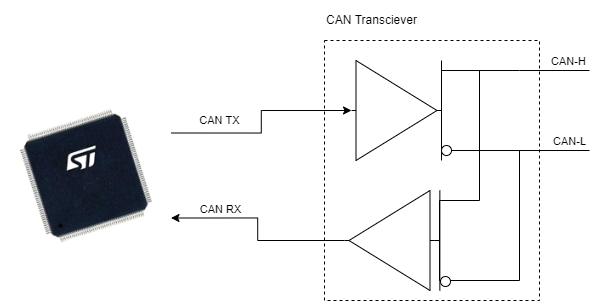
\includegraphics[width=0.5\textwidth]{img/microcontrolador_transciever.png}    
    \caption{El periférico embebido en el microcontrolador, a través del transciever, puede interactuar con el bus CAN.}
    \label{fig:microcontrolador_transciever}
\end{figure}

El protocolo CAN define dos estados para el bus, \textit{recessive} y \textit{dominant}. Cuando no hay actividad en el bus, tanto la línea de CAN-H como la de CAN-L se encuentran a la misma tensión constante. Esto corresponde al estado \textit{recessive} y equivale a un 1 lógico. Cuando se quiere enviar un 0 lógico, el transciever del nodo transmisor fija la tensión de las líneas CAN-H y CAN-L de tal forma de generar una tensión diferencial $V_{CAN-H} - V_{CAN-L} \geq 1,5 V$. Esto se muestra en la figura \ref{fig:CAN_recessive_dominant}.

\begin{figure}[H]
    \centering
    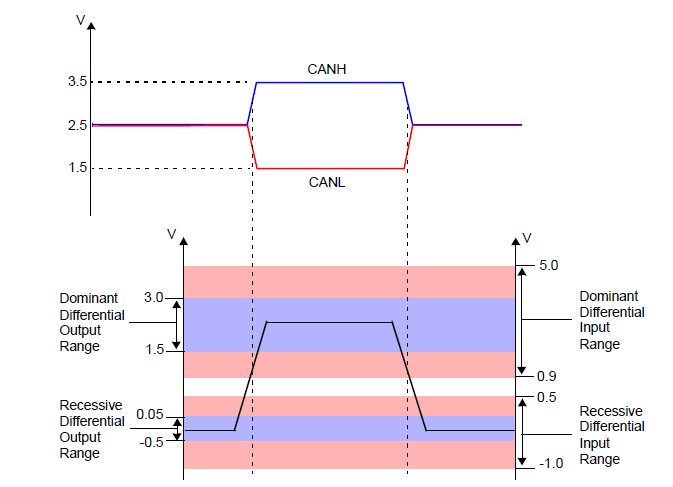
\includegraphics[width=0.7\textwidth]{img/CAN_recessive_dominant.png}
    \caption{Se muestran los estados recessive y dominant del bus CAN y sus equivalentes lógicos.}
    \label{fig:CAN_recessive_dominant}    
\end{figure}

Los nodos solamente actúan sobre el bus cuando quieren fijar un estado \textit{dominant}. Cuando se quiere fijar un estado \textit{recessive}, no se actúa sobre el bus ya que este es su estado por defecto. Esto lo que permite es que varios nodos puedan actuar al mismo tiempo. En caso de que esto suceda, el estado \textit{dominant} (de allí su nombre) predominará sobre el estado \textit{recessive}. Esto es lo que permite implementar el mecanismo de acceso al bus por prioridades.\\

La interfaz CAN se compone del transciever, su comunicación con el microcontrolador y el conector. En cuanto al transciever, se trata de un componente que es ampliamente utilizado en la electrónica automotriz, por lo que hay mucha disponibilidad. Existen transcievers que utilizan distintos niveles de tensión en sus salidas. La gran mayoría de los componentes de la computadora de vuelo utilizan tensiones de 3,3 V para su funcionamiento, por lo que se buscó algún transciever para esta tensión. El componente seleccionado es el SN65HVD230 de Texas Instruments \cite{SN65VHD230}, el cual es compatible con la especificación de capa física de CAN, ISO 11898-2. Este cuenta con una protección por exceso de tempertura, donde el componente pone sus salidas CAN-H y CAN-L en alta impdeancia, de manera de no perturbar al resto de los nodos. Por otro lado cuenta con una funcionalidad que permite detectar si el transciever fue desconectado del bus, fijando un estado alto constante en su salida RX hacia el \textit{controller}, informándole de la situación.\\

El transciever seleccionado además cuenta con un terminal que permite controlar el tiempo de crecimiento y de decrecimiento de las líneas CAN-H y CAN-L. Al realentizar el tiempo de crecimiento en las líneas CAN-H y CAN-L, se atenúa el contenido armónico de las más altas frecuencias, disminuyendo emisiones. Se coloca un resistor de $10 \ k\Omega$ en el terminal 8 denominado \textit{Rs}. Según la hoja de datos, esto corresponde a un slew-rate de $15 \ V / \mu s$.\\

La especificación de la capa física de CAN no define un conector. Se buscó seleccionar alguno que no ocupe demasiado espacio al ser montado en el PCB. En \cite{CiAconnector} se mencionan algunas recomendaciones de conectores. Este es un documento publicado por la organización internacional sin fines de lucro, \textit{CAN in Automation}, que se dedica a publicar recomendaciones y especificaciones relacionadas al uso del bus CAN. Dentro de las opciones que da este documento, se buscó alguno que tenga dimensiones razonables a lo requerido para la placa. De entre todas las opciones se seleccionó el connector que corresponde a la especificación de un protocolo CAN desarrollado para ser usado en drones, DroneCAN \cite{DroneCAN}, el conector JST GH 4. Por cuestiones de disponibilidad, se seleccionó otro componente similar a este y que es del mismo fabricante de otros de los conectores utilizados para la computadora de vuelo, los DF-13 de Hirose. Estos conectores son pequeños, por lo que no ocupan demasiado espacio en la placa.\\

En cuanto al circuito implementado, se tomó como punto de partida las recomendaciones de la hoja de datos del trasnciever SN65HVD230. Este recomienda el agregado de capacitores de desacople en las líneas de alimentación. Además, se agregaron resistores en serie con las líneas de CAN RX y CAN TX, es decir, en las pistas que llevan las señales que van desde el controller al transciever y viceversa. Esto se hizo como medida preventiva para amortiguar las señales, en caso de que estas presenten sobrepicos en las conmutaciones. A priori se fijan en $0 \ \Omega$ y se modificarán de ser necesario. El circuito completo de la interfaz CAN puede encontrarse en el \nameref{appendix:circuito_esquematico}.

\textbf{{\color{red} COMPLETAR EL ANÁLISIS DEL MODELO DE PARÁMETROS CONCENTRADOS, PARA LAS PISTAS CAN-TX Y CAN-RX, PARA CALCULAR EL EVENTUAL RESISTOR EN SERIE.}}

%\subsubsection{Circuito de Alimentación}
\subsection{Circuito de Alimentación}

Para alimentar el microcontrolador y los demás componentes, se incluye una fuente de alimentación de $3.3 \ V$. En las primeras dos versiones de la computadora de vuelo, desarrolladas por el LAR en trabajos anteriores, se integró una fuente conmutada de salida $5 \ V$ junto con un regulador lineal de $3.3 \ V$. A partir de la tercera versión, esta fuente conmutada se eliminó dejando solamente el regulador lineal de $3.3 \ V$ \cite{garberoglio2019diseno}. El motivo principal fue reducir las dimensiones de la placa y simplificar el diseño. Siguiendo esta misma línea, la fuente conmutada tampoco se incluyó en este trabajo. Se incorporó un conector, de manera de poder alimentar la placa utilizando una fuente externa de $5 \ V$.\\

El circuito implementado se comprende del regulador lineal, junto con capacitores de entrada y de salida. Para la selección del componente se buscó un regulador que sea de grado automotriz, por cuestiones de confiabilidad ya mencionadas, pero además se buscó un componente con un encapsulado SOT-223-3, figura \ref{fig:sot_223_3}. En el mercado local puede encontrarse una gran variedad de reguladores con este encapsulado, pensando en la necesidad de modificar el circuito, utilizando otro regulador o en caso de que haya que reemplazarlo.\\

\begin{figure}[H]
    \centering
    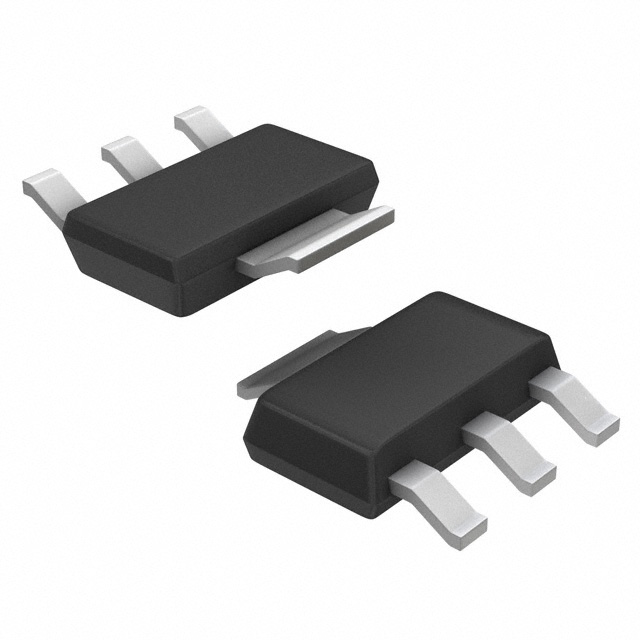
\includegraphics[width=0.3\textwidth]{img/sot_223_3.png}
    \caption{Encapsulado SOT-223-3 seleccionado para el regulador lineal. El terminal de mayor tamaño se encuentra conectado al terminal de tensión de salida, $3.3 \ V$.}
    \label{fig:sot_223_3}
\end{figure}

El chip seleccionado es el ZLDO1117QG33TA de DIODES Incorporated \cite{ZLDO1117QG33TA}, un regulador low-dropout de grado automotriz. Se siguió el circuito recomendado por la hoja de datos del fabricante, donde se coloca un capacitor a la entrada del regulador y otro en su salida.\\

La principal función del capacitor de entrada es la de proveer corriente al regulador, en caso de que ocurra un escalón en la corriente consumida por la carga del regulador \cite{TOSHIBALDO}. Este capacitor ayuda a mantener la tensión de entrada del regulador, en caso de que la fuente conectada a la entrada del regulador presente un drop-out. Se seleccionó un capacitor cerámico multicapa de valor $4.7 \ \mu F$. Este tipo de capacitores tienen una ESR muy baja, lo que permite que se descarguen rápido, en caso de que tengan que entregar carga para mantener la tensión de entrada en el regulador.\\

En cuanto al capacitor de salida, este cumple una doble función. Por un lado, aportar a la regulación de línea. Este parámetro es importante teniendo en cuenta que el regulador se utiliza para alimentar un circuito digital, donde aparecen muchas variaciones de corriente. En el caso en el que ocurra un cambio brusco de la corriente de salida del regulador, el capacitor de salida se descargará en parte, para intentar mantener la tensión de salida en un valor constante. Por otro lado, este capacitor también es utilizado para la compensación del regulador \cite{TOSHIBALDO}. En la figura \ref{fig:LDO_diagrama_bloques} se muestra un diagrama en bloques simplificado para un regulador lineal, donde puede verse que se trata de un sistema a lazo cerrado.

\begin{figure}[H]
    \centering
    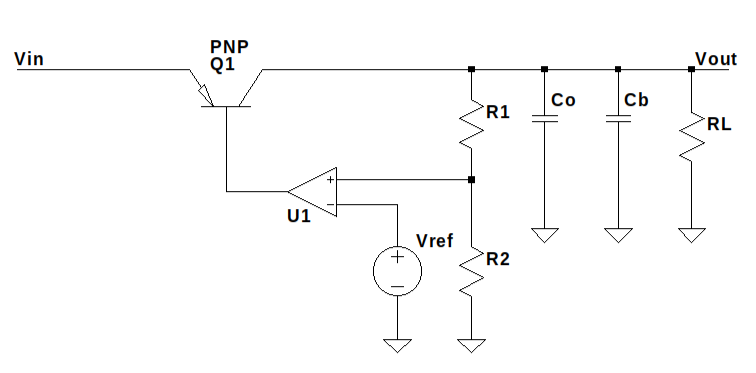
\includegraphics[width=0.7\textwidth]{img/LDO_diagrama_bloques.png}
    \caption{Diagrama en bloques de un regulador lineal. Este se compone de un transistor de paso, un amplificador de error, una tensión de referencia y un bloque realimentador, formado por $R_1$ y $R_2$. En el diagrama además se muestra $R_L$ que simboliza una carga resistiva y dos capacitores $C_o$ y $C_b$. Estos elementos forman un circuito a lazo cerrado que estabiliza la tensión de salida $V_{out}$.}
    \label{fig:LDO_diagrama_bloques}    
\end{figure}

Para analizar la ganancia de lazo, se plantea el esquema de realimentación en la figura \ref{fig:LDO_esquema_realimentacion}. Para el transistor de paso, se utiliza su modelo de pequeña señal. 

\begin{figure}[H]
    \centering
    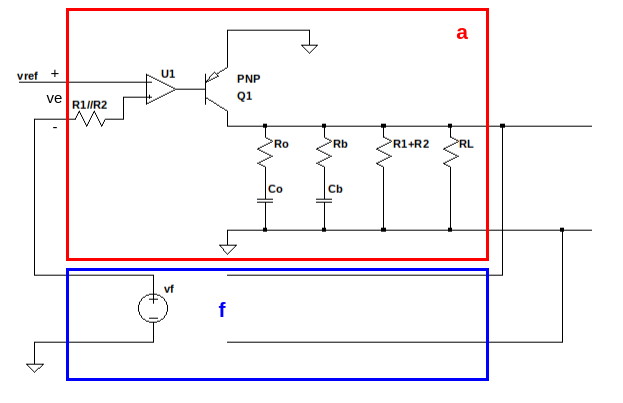
\includegraphics[width=0.8\textwidth]{img/LDO_esquema_realimentacion.png}
    \caption{Circuito equivalente para analizar la realimentación del regulador lineal. La tensión $v_{in}$ se pasiva ya que se analiza el circuito en el punto de operación.}
    \label{fig:LDO_esquema_realimentacion}    
\end{figure}

Se trata de un esquema que muestrea tensión y suma tensión. El bloque \textit{f} es tal que cumple con la relación de la ecuación \eqref{eq:LDO_bloque_f}. En cuanto al bloque \textit{a}, la transferencia corresponde a la ecuación \eqref{eq:LDO_bloque_a}, donde se ha asumido que $R_b \rightarrow 0$ por ser la ESR de un capacitor cerámico multicapa, $R_L \ll r_o$ y $R_L \ll (R_1+R_2)$. Además, se asume que $R_o \ll R_L$.

\begin{subequations}
    \begin{align}
        v_f &= f \ v_o\\
        f &= \frac{R_2}{R_1 + R_2} \label{eq:LDO_bloque_f}
    \end{align}
\end{subequations}

\begin{subequations}
    \begin{align}
        v_o &= a \ v_{ref}\\
        a &= A_v(s) g_m  R_L \frac{1 + s C_o R_o}{\left( 1 + s C_o  R_L \right)  \left( 1 + s C_b R_o \right)} \label{eq:LDO_bloque_a}
    \end{align}
\end{subequations}

La transferencia $A_v(s)$ corresponde al amplificador de error y se modela como de un polo simple. Juntando los bloques $a$ y $f$ puede obtenerse la ganancia de lazo para analizar la estabilidad, ecuación \eqref{eq:LDO_ganancia_lazo}. Esta se compone de 3 polos y 1 cero. Este último junto con uno de los polos dependen directamente del valor $R_o$, es decir, la ESR del capacitor de salida $C_o$. En caso de que la ESR sea muy pequeña, se obtiene un sistema con dos polos. Si bien este es estable, su margen de fase es muy pequeño. Esto se traduce en respuestas a transitorios con oscilaciones, por ejemplo causados por variaciones en la corriente de salida del LDO. En la figura \ref{fig:LDO_ganancia_lazo_1} se muestra la comparación entre el sistema compensado y sin compensación.

\begin{equation}
    af = \frac{R_2}{R_1+R_2} A_v(s) g_m  R_L \frac{1 + s C_o R_o}{\left( 1 + s C_o R_L \right) \left( 1 + s C_b R_o \right)}
    \label{eq:LDO_ganancia_lazo}
\end{equation}

\begin{figure}[H]
    \centering
    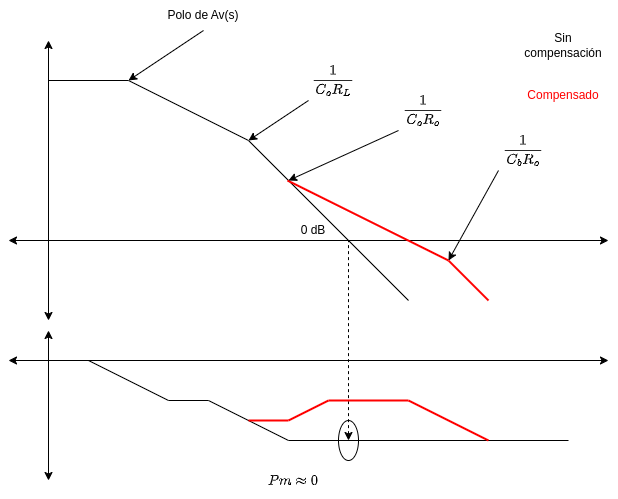
\includegraphics[width=0.7\textwidth]{img/LDO_ganancia_lazo_1.png}
    \caption{Se muestra un gráfico representativo de la ganancia de lazo de un LDO. En rojo se destaca cómo varía la ganancia de lazo con el agregado de un polo y un cero.}
    \label{fig:LDO_ganancia_lazo_1}    
\end{figure}

Al agregar los capacitores de salida $C_o$ y $C_b$, se forma un compensador en adelanto que incrementa el margen de fase. De este gráfico se desprende que si la resistencia ESR del capacitor de salida $C_o$ es muy pequeña, luego tanto el polo en $1/(C_b R_o)$ como el cero $1/(C_o R_o)$ se desplazan hacia la derecha en frecuencia y no funcionan como compensador en adelanto. Por otro lado, si la ESR es muy grande, el polo y el cero se desplazan a la izquierda y tampoco funcionarán como compensador \cite{SLVA072}. De aquí se desprende el hecho de que la elección del valor de ESR debe ser adecuada.\\

El fabricante recomienda un valor de ESR entre $0.05 \ \Omega$ y $0.5 \  \Omega$, de un valor de por lo menos $4.7 \ \mu F$. Los capacitores MLCC típicamente tienen ESR muy bajas, del orden de unos pocos $m \Omega$. Debido a esto, se selecciona un capacitor de tantalio para el capacitor de salida \cite{AN1482}, que suelen excibir una ESR mayor a la de los MLCC. El componente seleccionado es el T491A106K016ATAUTO de KEMET. Al igual que Murata, este proveedor ofrece curvas de las características del componente.\\

Como fue ya fue mencionado, se incorpora un conector que permite adosar una fuente externa. El conector se seleccionó pensando en utilizar algunos módulos típicos para drones y vehículos aéreos \cite{HolybroPM02PowerModule}. Estos módulos, además de las líneas de tensión y de retorno, tienen dos líneas más que entregan información del estado de la batería. Estas son señales analógicas que informan acerca de la tensión y la corriente de la batería. La computadora de vuelo sensa dicha información utilizando entradas analógicas. Además, se incluyen dos filtros pasa bajos, uno por cada señal analógica. Estos pueden encontrarse en el apéndice.\\

La placa además cuenta con un puerto micro USB B a través del cual también puede alimentarse la placa. Tanto la línea de $5 \ V$ del conector USB, como la del conector de alimentación principal, tienen en serie un diodo schottky. Estos diodos fuerzan a que las corrientes solamente fluyan desde las entradas de $5 \ V$ hacia el regulador. El circuito completo puede encontrarse en el \nameref{appendix:circuito_esquematico}.\\

%\subsubsection{Micro SD}
\subsection{Micro SD}

\textbf{{\color{red} COMPLETAR}}

%\subsubsection{Interfaz USB}
\subsection{Interfaz USB}

\textbf{{\color{red} COMPLETAR}}

%\subsubsection{Micro Switch}
\subsection{Micro Switch}

\textbf{{\color{red} COMPLETAR}}

%\subsubsection{LEDs Indicadores}
\subsection{LEDs Indicadores}

\textbf{{\color{red} COMPLETAR}}

%\subsubsection{Conector para Módulo GPS}
\subsection{Conector para Módulo GPS}

\textbf{{\color{red} COMPLETAR}}

%\subsubsection{Conectores para Salidas de PWM}
\subsection{Conectores para Salidas de PWM}

\textbf{{\color{red} COMPLETAR}}

%\subsubsection{Conector para Programación por SWD}
\subsection{Conector para Programación por SWD}

\textbf{{\color{red} COMPLETAR}}

%\subsubsection{Conector para Control por Radio}
\subsection{Conector para Control por Radio}

\textbf{{\color{red} COMPLETAR}}

\subsection{Desarrollo del PCB}

\textbf{{\color{red} COMPLETAR}}

\subsubsection{Requerimientos de Manufacturabilidad}

\textbf{{\color{red} COMPLETAR}}

% Acá poner el motivo por el que está todo en una sola cara.

% También justificar el espesor del cobre y las vías pasantes en ves de vías ciegas.

\subsubsection{Requerimientos de layout del sensor IMU}

El sensor IMU tiene ciertos requerimientos particulares que deben cumplirse. En primera instancia se buscó ubicar al componente lo más centrado posible en el PCB. De esta forma, la terna solidaria al sensor coincidirá con la terna solidaria a todo el vehículo en el que se utilice la placa. Esto ahorra cuestiones de cómputo que modifiquen la terna de referencia respsecto de la cual se obtengan las lecturas. \textbf{{\color{red} Completar qué tan corrida quedó la IMU del centro de la placa}}\\

Se siguieron una serie de guías y recomendaciones que tienen como objetivo minimizar el estrés sobre el componente \cite{IMUpcb_1} \cite{IMUpcb_2} \cite{IMUpcb_3}. Esto debido a que, como la IMU es un sistema electromecánico, el estrés puede alterar las mediciones que esta realice, o incluso un alto nivel de estrés puede llegar a dañar el componente. Se enumeran algunas de esas recomendaciones:

\begin{itemize}
    \item Montar la IMU lejos de orificios de montaje para el PCB, lejos de orificios para colocar tornillos y lejos de componentes como pulsadores y conectores. Para el caso de un pulsador, por ejemplo, al presionarlo esto genera una presión sobre el PCB. Si la IMU se encuentra muy cerca del pulsador, dicha presión puede llegar a afectar la zona donde se encuentra la IMU, alterando las mediciones. Los orificios deben estar a una distancia de por lo menos 2 mm del sensor.
    \item Montar la IMU lejos de los bordes del PCB.
    \item No ubicar test points ni conectores debajo de la IMU, es decir, en la otra cara del PCB. El conectar y desconectar continuamente puede dañar el componente.
    \item El layout del circuito debe ser lo más simétrico posible. No es necesario utilizar pistas de un tamaño diferente para las líneas de alimentación, ya que su consumo es muy bajo.
    \item No pasar pistas debajo de la IMU.
    \item No ubicar vías debajo del componente. El área debajo de este debe definirse como keepout area.
\end{itemize}

La imagen de la figura \ref{fig:IMU_recomendaciones_layout} resume algunas de estas recomendaciones. Lo que se observa es que las pistas del sensor son simétricas. Por más de que algunos terminales de la IMU no se utilicen, se recomienda que el routeo sea simétrico. Durante el proceso de soldadura, el estaño presente en los distintos pads del componente generará una tensión que tratará de atraer al componente hacia este. Si el routeo no es simétrico, es posible que el sensor no quede centrado, lo que resultaría en un grave problema durante el uso de la computadora de vuelo.

\begin{figure}[H]
    \centering
    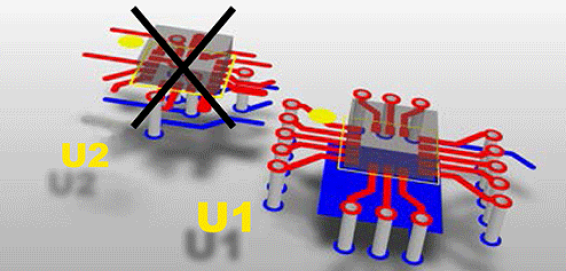
\includegraphics[width=0.5\textwidth]{img/IMU_recomendaciones_layout.png}
    \caption{Se muestran dos ejemplos de layout de una IMU. El layout U2 no sigue las recomendaciones mencionadas, mientras que U1 sí. La imagen se extrajo de \cite{IMUpcb_3}.}
    \label{fig:IMU_recomendaciones_layout}
\end{figure}

\subsubsection{Layout del Regulador Lineal}

\textbf{{\color{red} COMPLETAR}}

\subsubsection{Comunicación con el Slot para Tarjeta Micro SD}

% Length matching e impedancia característica. Mencionar todo lo que tengo de la especificación de microSD. Tengo muchísimo de esto.

\textbf{{\color{red} COMPLETAR}}

\subsubsection{Comunicación USB}

% Impedancia característica de la pista diferencial, de la especificación.

\textbf{{\color{red} COMPLETAR}}